\documentclass[a4paper,oneside]{book}
\usepackage{geometry}
 \geometry{
 a4paper,
 total={170mm,257mm},
 left=20mm,
 top=20mm,
 }
\bibliographystyle{plain}
\usepackage{indentfirst}
\usepackage{csquotes}
\usepackage{graphicx}
\usepackage{wrapfig}
\graphicspath{ {./src/} }
\usepackage{hyperref}
\hypersetup{
    colorlinks=true,
    linkcolor=blue,
    filecolor=magenta,
    urlcolor=cyan,
}
\usepackage[linguistics]{forest}
\usepackage{ragged2e}
\usepackage{array}
\usepackage{booktabs}
\newcolumntype{R}[1]{>{\RaggedLeft\arraybackslash}p{#1}}
\newcolumntype{C}[1]{>{\Centering\arraybackslash}p{#1}}
\usepackage{amsmath}
\newcommand{\boxalign}[2][0.97\textwidth]{
 \par\noindent\tikzstyle{mybox} = [draw=black,inner sep=6pt]
 \begin{center}\begin{tikzpicture}
  \node [mybox] (box){%
   \begin{minipage}{#1}{\vspace{-5mm}#2}\end{minipage}
  };
 \end{tikzpicture}\end{center}
}
\usepackage[boxed, ruled]{algorithm2e}
%% This declares a command \Comment
%% The argument will be surrounded by /* ... */
\SetKwComment{Comment}{/* }{ */}
\usepackage{multicol}
\usepackage{listings}
\lstset{
basicstyle=\small\ttfamily,
breaklines=true
}
\usepackage{longtable}

\begin{document}

\clearpage
%% temporary titles
% command to provide stretchy vertical space in proportion
\newcommand\nbvspace[1][3]{\vspace*{\stretch{#1}}}
% allow some slack to avoid under/overfull boxes
\newcommand\nbstretchyspace{\spaceskip0.5em plus 0.25em minus 0.25em}
% To improve spacing on titlepages
\newcommand{\nbtitlestretch}{\spaceskip0.6em}
\pagestyle{empty}
\begin{center}
    \bfseries
    \nbvspace[1]
    \Huge
    {\nbtitlestretch\huge
        Autograd for Algebraic Expression}

    \nbvspace[1]
    \normalsize

    Project 2 Report\\
    Fundamental of Data Structure (2023 Fall)\\
    Zhejiang University
    \nbvspace[1]
    \small BY\\
    \Large Author Name\\[0.5em]
    \footnotesize Student ID: \\
    Teacher: HongHua Gan

    \nbvspace[2]
    Accomplished on October 27, 2023
    \nbvspace[3]
    \normalsize

    Made\\
    \large
    With \LaTeX
    \nbvspace[1]
\end{center}

\chapter*{Declaration}

I hereby declare that all the work done in this project titled ``Autograd for Algebraic Expression'' is of my independent effort.

\tableofcontents

\chapter{Introduction}

This chapter gives a brief introduction to the project, including the problem
description, problem background, and the context-free grammar of the expression.

\section{Problem Description}

In this project, we are going to implement an autograd system for analysing and differentiating algebraic expressions. Given a mathematical expression in the form of a string, the task is to develop a program that can automatically analyse the structure of the expression and evaluate its derivative with respect to every variable appearing in the expression. The program should be able to handle expressions with multiple variables, support basic mathematical operations, and accurately compute its derivative.

\section{Problem Background}

Autograd, short for automatic differentiation, is a technique used in computational mathematics and machine learning to efficiently compute derivatives of functions. It plays a crucial role in optimization algorithms, neural network training~\cite{paszke2017automatic}, and various scientific computations.

By implementing such a system, it becomes possible to automate the evaluation and differentiation of algebraic expressions, saving time and effort in various mathematical and scientific applications.

\section{Context-free Grammar of the Expression}

The expression defined in the problem can be more systematically described using a context-free grammar to guide the translation from string to expression analyse tree.

A context-free grammar consists of three parts: a set of \textbf{terminal symbols} (represent in bold), a set of \textit{non-terminal symbols} (represent in italics), and a set of production rules. Terminal symbols are the basic symbols of the language, while non-terminal symbols are symbols that can be derived into terminal symbol strings. Production rules describe how non-terminal symbols can be constructed from terminal and non-terminal symbols. One of the non-terminal symbols is designated as the start symbol, which is the symbol that can be derived into the entire language.

Based on the problem description, the terminal symbols of the expression are defined as follows:

\begin{table}[!ht]
    \centering
    \caption{Terminal of the Expression}\label{tab:terminals}
    \begin{tabular}{C{0.1\textwidth} C{0.2\textwidth}  p{0.6\textwidth}}
        \toprule
        Symbol Name       & Example                   & Description                                                  \\
        \midrule
        \textbf{digits}   & \verb|19 1|               & A sequence of digits.                                        \\
        \textbf{variable} & \verb|x xyz|              & A sequence of lowercase letters that is not a function name. \\
        \textbf{operator} & \verb|+ - * / ^|          & An operator.                                                 \\
        \textbf{fun1}     & \verb|sin cos tan exp ln| & A function with one argument.                                \\
        \textbf{fun2}     & \verb|pow log|            & A function with two arguments.                               \\
        \textbf{bracket}  & \verb|( )|                & A bracket.                                                   \\
        \textbf{comma}    & \verb|,|                  & A comma.                                                     \\
        \bottomrule
    \end{tabular}
\end{table}

\begin{wrapfigure}{r}{0.3\textwidth}
    \caption{Non-terminals and their productions}\label{fig:production}
    \boxalign[0.3\textwidth]{
        \begin{align*}
            \textit{factor} & \to \textbf{digits}                                                               \\
                            & \mid\  \textbf{-} \textit{\ factor}                                               \\
                            & \mid\  \textbf{+} \textit{\ factor}                                               \\
                            & \mid\  \textbf{variable}                                                          \\
                            & \mid\  \textbf{fun1} \textbf{(} \textit{expr} \textbf{)}                          \\
                            & \mid\  \textbf{fun2} \textbf{(} \textit{expr} \textbf{,} \textit{expr} \textbf{)} \\
                            & \mid\  \textbf{(} \textit{expr} \textbf{)}                                        \\
            \textit{pow}    & \to \textit{factor}                                                               \\
                            & \mid\  \textbf{-} \textit{\ pow}                                                  \\
                            & \mid\  \textbf{+} \textit{\ pow}                                                  \\
                            & \mid\  \textit{pow} \textbf{\ \^{}\  } \textit{factor}                            \\
            \textit{term}   & \to \textit{pow}                                                                  \\
                            & \mid\  \textbf{-} \textit{\ term}                                                 \\
                            & \mid\  \textbf{+} \textit{\ term}                                                 \\
                            & \mid\  \textit{term} \textbf{\ *\ } \textit{pow}                                  \\
                            & \mid\  \textit{term} \textbf{\ /\ } \textit{pow}                                  \\
            \textit{expr}   & \to \textit{term}                                                                 \\
                            & \mid\  \textit{expr} \textbf{\ +\ } \textit{term}                                 \\
                            & \mid\  \textit{expr} \textbf{\ -\ } \textit{term}
        \end{align*}}
\end{wrapfigure}

The approach to defining non-terminal symbols is as follows:

\begin{itemize}
    \item A non-terminal symbol should be defined for each level of operator precedence.
    \item A terminal symbol should be defined to represent factors that cannot be separated by operators, such as variables, mathematical functions, etc.
\end{itemize}

The expression mentioned in the problem description contains three different levels of operators, so I defined four non-terminal symbols. The resulting four non-terminal symbols and their production rules can be seen in Figure~\ref{fig:production}, and the associativity of the operators is also indicated in the production rules. The start symbol of the grammar is \textit{expr}.

\begin{wrapfigure}{l}{0.35\textwidth}
    \caption{Parse tree of \texttt{sin(x+1)*2}}\label{fig:parse_tree}
    \fbox{
        \begin{forest}
            [\textit{expr}
                [\textit{term}
                    [\textit{term}
                        [\textit{pow}
                            [\textit{factor}
                                [\textbf{fun1}
                                    [\textbf{sin}]
                                ]
                                [\textbf{(}]
                                [\textit{expr}
                                    [\textit{term}
                                        [\textit{pow}
                                            [\textit{factor}
                                                [\textbf{variable}
                                                    [\textbf{x}]
                                                ]
                                            ]
                                        ]
                                    ]
                                    [\textbf{+}]
                                    [\textit{term}
                                        [\textit{pow}
                                            [\textit{factor}
                                                [\textbf{constant}
                                                    [\textbf{1}]
                                                ]
                                            ]
                                        ]
                                    ]
                                ]
                                [\textbf{)}]
                            ]
                        ]
                    ]
                    [\textbf{*}]
                    [\textit{pow}
                        [\textit{factor}
                            [\textbf{constant}
                                [\textbf{2}]
                            ]
                        ]
                    ]
                ]
            ]
        \end{forest}}
\end{wrapfigure}

Now let's have a look at the parse tree of the expression \verb|sin(x + 1) * 2|:

\begin{itemize}
    \item The root of the tree is the start symbol \textit{expr}.
    \item Match the production rule of \textit{expr} with the input string, but found it could only be a \textit{term}.
    \item Match the production rule of \textit{term} with the input string, and succeeded with pattern \textit{term} \textbf{*} \textit{pow}.
    \item Recursively match the production rule of \textit{term} and \textit{pow} to the left and right sub-string of the above pattern.
\end{itemize}

The parsed tree is shown in Figure~\ref{fig:parse_tree}.

\chapter{Algorithm Specfication}
\label{chap:algorithm}

This chapter gives description of the main program and the algorithms used in each part.

\section{Architecture of the Program}

The program structure of the autoGrad program is similar to that of a compiler. The expression in string format goes through a lexical analyser and a syntax parser, continuously abstracting it into higher-level expressions and finally generating an expression tree. The optimizer and differentiator operate on the expression tree data structure. The collaboration between different modules of the program is illustrated in the following diagram:

\begin{figure}[!ht]
    \caption{Data flow of the program}
    \centering
    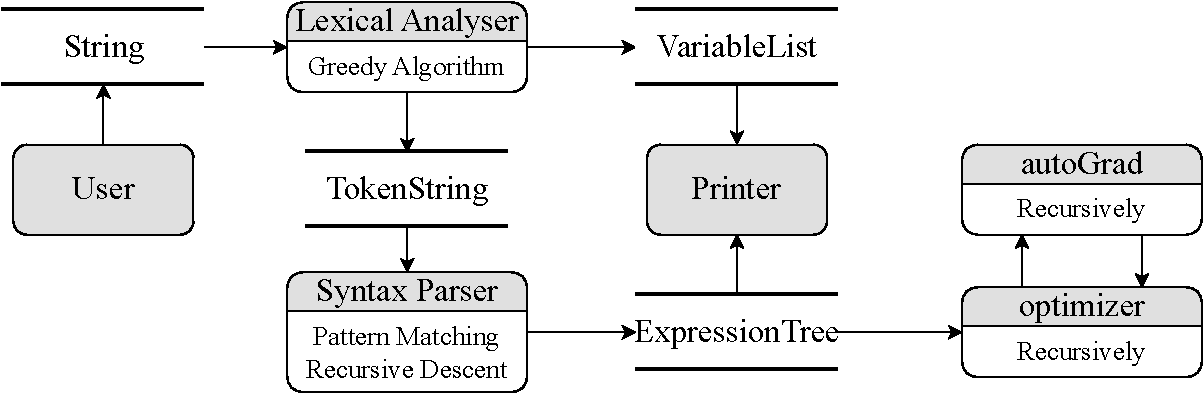
\includegraphics[width=0.8\textwidth]{src/dataflow.drawio.pdf}
\end{figure}

\section{Lexcial Analyser}

\begin{wrapfigure}{r}{0.3\textwidth}
    \caption{Lexcial Analyser}
    \centering
    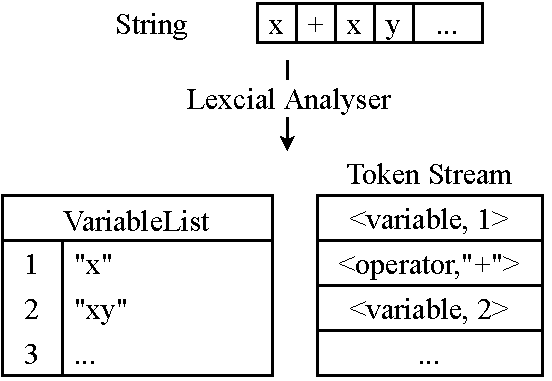
\includegraphics[width=0.3\textwidth]{src/token_varlist.drawio.pdf}
\end{wrapfigure}

Tokens are terminals of the expression. Lexcial analyser uses a greedy algorithm to match the longest possible token from the input string. It converts the string into a token stream, which is then passed to the syntax parser.

\subsection{\texttt{String}, \texttt{Token} and \texttt{VariableList} Data Structure}

The \verb|String| type is just a wrapper type used for convenient input and keeping track of the current position during parsing. It dynamically allocates memory based on the input size. Each time the lexer is called on a \verb|String|, it updates the position that has been read in the string.

The \verb|token| type is defined as a structure with two fields: \verb|type| and \verb|value|.\ \verb|type| is an enumeration type that represents the type of the token (see~\ref{tab:terminals}), and \verb|value| is an int type that represents the value of the token.

VariableList is a structure that stores the names of variables in the expression. It is implemented as an \verb|char*| array for convenient add and query operations. Value of a variable token is the index of the variable in the VariableList. There is also an index array named \verb|dictOrder| that is sorted by dictionary order. It is used to print the variable list in alphabetical order.

\begin{table}[!h]
    \caption{API of \texttt{Token} and \texttt{VariableList} Type}
    \resizebox{\textwidth}{!}{
        \begin{tabular}{rrll}
            \toprule
            Type          & Name               & Arguments                                 & Description                                  \\
            \midrule
            String*       & getString          & (void)                                    & Read one line from stdin and return a string \\
            VariableList* & createVariableList & (void)                                    & Create a variable list object                \\
            int           & querySymbol        & (VariableList *list, char *symbol)        & Query the index of a variable in the list    \\
            int           & addSymbol          & (VariableList *list, char *symbol)        & Add a variable to the list and return index  \\
            void          & printVariableList  & (VariableList *list)                      & Print variable list object                   \\
            void          & freeVariableList   & (VariableList *list)                      & Free variable list object                    \\
            Token         & getToken           & (String *s, VariableList *list)           & Get a token from the string                  \\
            void          & printTokens        & (Token *tokens, int num, VariableList *v) & Print token stream                           \\
            \bottomrule
        \end{tabular}
    }
\end{table}

\subsection{Greedy Matching Algorithm}

The algorithm is implemented in the function \verb|getToken()|. It takes a string and a variable list as input, and returns the next token in the string.

\begin{algorithm}[H]
    \caption{Greedy Matching Algorithm}\label{alg:1}
    \DontPrintSemicolon
    \KwIn{A string $s$ and a variable list $v$}
    \KwOut{The next token in the string}
    \BlankLine
    $token \gets \text{NULL}$\;
    \While{$s$ is not empty}{
        $token \gets \text{NULL}$\;
        \For{$i \gets 0$ \KwTo $n$}{
            \If{$s[0:i]$ is a token}{ \Comment*[r]{Greedy match token}
                $token \gets s[0:i]$\;
            }
        }
        \If{$token$ is \text{NULL}}{
            \Return{NULL}\;
        }
        \Else{
            $s \gets s[i:]$\; \Comment*[r]{Update string}
            \If{$token$ is a variable}{
                $index \gets \text{querySymbol}(v, token)$\; \Comment*[r]{Maintain variable list}
                \If{$index$ is \text{NULL}}{
                    $index \gets \text{addSymbol}(v, token)$\;
                }
                $token \gets \text{createToken}(\text{VARIABLE}, index)$\;
            }
            \Return{$token$}\;
        }
    }
\end{algorithm}

\section{Syntax Parser}

\begin{wrapfigure}{r}{0.5\textwidth}
    \caption{Syntax Parser}
    \centering
    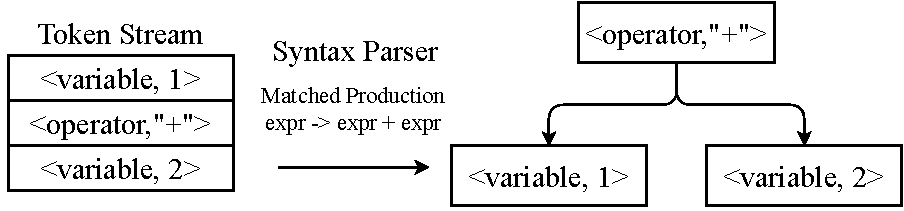
\includegraphics[width=0.5\textwidth]{src/syntax.drawio.pdf}
\end{wrapfigure}

Syntax parser receives a token stream from the lexical analyser and generates an expression tree. It uses a recursive descent algorithm to parse the token stream. The algorithm is implemented in the function \verb|parse()|.

\subsection{\texttt{Node} Data Structure}

The expression tree is implemented as a binary tree. Each node of the tree is a structure with three fields: \verb|token|, \verb|left| and \verb|right|.\ \verb|Token| is described in the previous section.\ \verb|left| and \verb|right| are pointers to the left and right child of the node.

In the expression tree, the internal nodes are operators and functions, and the leaf nodes are variables and digits. Other types of tokens is just used for parsing and will not appear in the expression tree.

\begin{table}[!h]
    \caption{API of \texttt{Node} Type}
    \resizebox{\textwidth}{!}{
        \begin{tabular}{rrll}
            \toprule
            Type  & Name            & Arguments                       & Description                                             \\
            \midrule
            Node* & createNode      & (Token t, Node *a, Node *b)     & Create a node object                                    \\
            Node* & copyTree        & (Node *node)                    & Copy a node object recursively                          \\
            void  & printTree       & (Node *node, VariableList *v)   & Print node object                                       \\
            void  & freeNode        & (Node *node)                    & Free node object recursively                            \\
            int   & isBracketPaired & (Token *t, int start, int end)  & Check if brackets are paired                            \\
            Node* & parse           & (String *s, VariableList *list) & Wrapper function for getToken() and following functions \\
            Node* & exprParser      & (Token *t, int start, int end)  & Parse the token stream into an expression tree          \\
            Node* & termParser      & (Token *t, int start, int end)  & Parse the token stream into a term tree                 \\
            Node* & powParser       & (Token *t, int start, int end)  & Parse the token stream into a pow tree                  \\
            Node* & factorParser    & (Token *t, int start, int end)  & Parse the token stream into a factor tree               \\
            \bottomrule
        \end{tabular}
    }
\end{table}

\subsection{Pattern Matching and Recursive Descent Algorithm}

The algorithm is implemented in the function \verb|exprParser()|, \verb|termParser()|, \verb|powParser()| and \verb|factorParser()|. When the higher-priority parser function fails to parse the token stream or successfully matches a pattern, it will call the same-priority or lower-priority parser function to continue parsing the remaining portion of the token stream. The algorithm is described in the following block:

\begin{algorithm}[H]
    \caption{Recursive Descent Algorithm for non-terminal p}\label{alg:2}
    \DontPrintSemicolon
    \KwIn{A token stream $t$ and a variable list $v$}
    \KwOut{An expression tree}
    \BlankLine
    \emph{When p is not the lowest-priority parser}\;
    \If{$t$ applies to the production rule of p}{
        \Return{the expression tree}\;
    }
    \Else{
        \emph{Call the lower-priority parser function}\;
    }
    \BlankLine
    \emph{When p is the lowest-priority parser}\;
    \If{$t$ can't applies to the production rule of this parser}{
        \emph{Report error}\;
    }

\end{algorithm}

\section{Optimizer}

I implemented a simple optimizer that can simplify the expression tree by evaluating constant sub-expressions. The optimizer is implemented in the function \verb|constantOptimizer()|. It will recursively apply the following rules to the expression tree and return a \textbf{new} optimized tree.

\begin{multicols}{2}
    \begin{align*}
        0+\mathrm{f}(x)=\mathrm{f}(x)+0 =\mathrm{f}(x)-0              & =\mathrm{f}(x)                 \\
        0\cdot\mathrm{f}(x)=\mathrm{f}(x)\cdot0                       & =0                             \\
        0/\mathrm{f}(x)                                               & =0                             \\
        1^{\mathrm{f}(x)}=\mathrm{f}(x)^0                             & =1                             \\
        \ln(1)=\sin(0) =\tan(0)                                       & =0                             \\
        \log_{\mathrm{f}(x)} {\mathrm{f}(x)}                          & =1                             \\
        \mathrm{pow}(\mathrm{f}(x), 0)=\mathrm{pow}(1, \mathrm{f}(x)) & =1                             \\
        \mathrm{pow}(\mathrm{f}(x), \mathrm{f}(x))                    & =\mathrm{f}(x)^{\mathrm{f}(x)} \\
    \end{align*}\break
    \begin{align*}
        0-\mathrm{f}(x)                         & =-\mathrm{f}(x) \\
        1\cdot\mathrm{f}(x)=\mathrm{f}(x)\cdot1 & =1              \\
        \mathrm{f}(x)/1                         & =\mathrm{f}(x)  \\
        0^{\mathrm{f}(x)}                       & =0              \\
        \cos(0)=\exp(0)                         & =1              \\
        \log_{\mathrm{f}(x)} 1                  & =0              \\
        \mathrm{pow}(0, \mathrm{f}(x))          & =0              \\
        \mathrm{pow}(\mathrm{f}(x), 1)          & =\mathrm{f}(x)  \\
    \end{align*}
\end{multicols}

\begin{algorithm}[H]
    \caption{Optimizer Algorithm}\label{alg:3}
    \DontPrintSemicolon
    \KwIn{An expression tree $t$}
    \KwOut{An optimized expression tree}
    \BlankLine
    \If{$t$ has child}{
        Optimize child\;
    }
    Construct a new node $n$ following the rules\;
    \Return{$n$}\;
\end{algorithm}

As for implementation, the equations above is converted to a bunch of \verb|if| statements which is so diverse that I can't show them here. The details can be found in the function \verb|constantOptimizer()|.

\section{Differentiator}

For every node (including leaf), differentiator \verb|autoGrad| applies the following rules to the expression tree and return a \textbf{new} diffrentiated tree.

\begin{multicols}{2}
    \begin{align*}
        \ln({\mathrm{f}(x)})'  & = \frac{{\mathrm{f}'(x)}}{{\mathrm{f}(x)}}                 \\
        \sin({\mathrm{f}(x)})' & = {\mathrm{f}'(x)} \cdot \cos({\mathrm{f}(x)})             \\
        \cos({\mathrm{f}(x)})' & = -{\mathrm{f}'(x)} \cdot \sin({\mathrm{f}(x)})            \\
        \tan({\mathrm{f}(x)})' & = {\mathrm{f}'(x)} \cdot \frac{1}{\cos^2({\mathrm{f}(x)})} \\
        \exp({\mathrm{f}(x)})' & = {\mathrm{f}'(x)} \cdot \exp({\mathrm{f}(x)})
    \end{align*}\break
    \begin{align*}
        ({\mathrm{f}(x)} \pm {\mathrm{g}(x)})'     & = {\mathrm{f}'(x)} \pm {\mathrm{g}'(x)}                                                                                                                  \\
        ({\mathrm{f}(x)} \cdot {\mathrm{g}(x)})'   & = {\mathrm{f}'(x)} \cdot {\mathrm{g}(x)} + {\mathrm{f}(x)} \cdot {\mathrm{g}'(x)}                                                                        \\
        (\frac{{\mathrm{f}(x)}}{{\mathrm{g}(x)}})' & = \frac{{\mathrm{f}'(x)} \cdot {\mathrm{g}(x)} - {\mathrm{f}(x)} \cdot {\mathrm{g}'(x)}}{{\mathrm{g}(x)}^2}                                              \\
        ({\mathrm{f}(x)}^{{\mathrm{g}(x)}})'       & = {\mathrm{f}(x)}^{{\mathrm{g}(x)}} \cdot [{\mathrm{g}'(x)} \cdot \ln({\mathrm{f}(x)}) + \frac{{\mathrm{g}(x)} \cdot {\mathrm{f}'(x)}}{{\mathrm{f}(x)}}] \\
        \log_{\mathrm{f}(x)} {\mathrm{g}(x)}       & = \frac{{\mathrm{g}'(x)}}{{\mathrm{g}(x)} \cdot \ln({\mathrm{f}(x)})} - \frac{\ln({\mathrm{g}(x)}) \cdot {\mathrm{f}'(x)}}{{\mathrm{f}(x)} }
    \end{align*}
\end{multicols}

\begin{algorithm}[H]
    \caption{Differentiator Algorithm}\label{alg:4}
    \DontPrintSemicolon
    \KwIn{An expression tree $t$, a variable $x$}
    \KwOut{A differentiated expression tree}
    \BlankLine
    \Switch{$t$}{
        \Case{$t$ is a constant}{
            \Return{0}\;
        }
        \Case{$t$ is a variable}{
            \If{$t$ is $x$}{
                \Return{1}\;
            }
            \Else{
                \Return{0}\;
            }
        }
        \Other{
            Recursively construct a new node $n$ following the rules\;
            \Return{$n$}\;
        }
    }
\end{algorithm}

\section{Printer}

The printer is implemented in the function \verb|printTree()|. It will recursively print the expression tree in infix notation.

The printer must check the priority of the operator and the associativity of the operator to determine whether to print brackets. It also needs to check whether the operator satisfies the commutative law to determine whether to print brackets.

\begin{algorithm}[H]
    \caption{Printer Algorithm}\label{alg:5}
    \DontPrintSemicolon
    \KwIn{A node $n$ and a variable list $v$}
    \KwOut{Print the expression tree in infix notation}
    \BlankLine
    \If{$n$ is empty}{
        \Return\;
    }
    \Switch{$n$}{
        \Case{$n$ is a variable, function or digit}{
            Print\;
        }
        \Case{$n$ is an operator}{
            \If{Child of $n$ is lower-priority operator}{
                Print bracket\;
            }
            Print left child\;
            Print operator\;
            Print right child\;
            \If{Child of $n$ is lower-priority operator}{
                Print bracket\;
            }
            \If{$n$ dissatisfies the commutative law}{
                \If{right child is same type as $n$}{
                    Print bracket\;
                }
            }
        }
        \Other{
            Report error: invalid node in tree\;
        }
    }
\end{algorithm}

\chapter{Testing Results}

The program successfully passed all the test cases. Here I selected some test cases from my test suite to show the correctness of the program. A more complete test suite can be seen in Appendix~\ref{chap:raw_test_results}.

Selected test cases with their purpose, input, output and correctness are shown in Table~\ref{tab:test_results} below.

    \begin{longtable}{|c|p{3cm}|p{3.6cm}|p{3.6cm}|c|}
        \caption{Test Results}\label{tab:test_results} \\
\hline
 \multicolumn{5}{| c |}{Begin of Table}\\
\hline
        No.                                                              & Purpose                                               & Input                                                             & Output                                                                          & Correctness \\ \hline
 \endfirsthead

 \hline
 \multicolumn{5}{|c|}{Continuation of Table \ref{tab:test_results}}\\
\hline
        No.                                                              & Purpose                                               & Input                                                             & Output                                                                          & Correctness \\ \hline
 \endhead

 \hline
 \endfoot

 \hline
 \multicolumn{5}{| c |}{End of Table}\\
 \hline\hline
 \endlastfoot

        1  & Test cases that only contain constants.               & \lstinline!-1^2!                                                  & \lstinline![warning] No variable in expression: (-1)!                                     & Yes         \\ \hline
        2  & Test cases that only contain variables and constants. & \lstinline!a*b/(a-b)*a/b^2!                                       &
        \lstinline!a: ((((b*(a-b)-a*b)/(a-b)^2)*a+(a*b)/(a-b))*b^2)/(b^2)^2!\newline{}\lstinline!b: ((((a*(a-b)-(a*b)*(-1))/(a-b)^2)*a)*b^2-(((a*b)/(a-b))*a)*(b^2*(2/b)))/(b^2)^2! & Yes  \\ \hline
        3  & Test cases that contain mathematical functions.       & \lstinline!sin(x)+cos(x)+tan(x)+exp(x)+ln(x)+log(2, x)+pow(x, 2)! & \lstinline!x: cos(x)+(-1)*sin(x)+1/cos(x)^2+exp(x)+1/x+(ln(2)/x)/ln(2)^2+x^2*(2/x)! & Yes         \\ \hline
        4 & Test cases that contain variables with different names. & \lstinline!vlog+a+b+wxyz! & \lstinline!a: 1!\newline{}\lstinline!b: 1!\newline{}\lstinline!vlog: 1!\newline{}\lstinline!wxyz: 1! & Yes \\ \hline
        5 & Test cases that contain nested expressions, multiple variables and functions. & \lstinline!log(a,b)^2+sin(x)^2! & \lstinline!a: log(a,b)^2*((((-1)*(ln(b)/a))/ln(a)^2)*(2/log(a,b)))!\newline{}\lstinline!b: log(a,b)^2*(((ln(a)/b)/ln(a)^2)*(2/log(a,b)))!\newline{}\lstinline!x: sin(x)^2*(cos(x)*(2/sin(x)))! & Yes \\ \hline
        6 & Test cases that can be simplified. & \lstinline!x+x+x! & \lstinline!x: 3! & Yes \\ \hline
        7 & Large Size & \lstinline!a^a^a^a^a^a^a^a^a^a^a^a^a! & \lstinline!a: a^(a^(a^(a^(a^(a^(a^(a^(a^(a^(a^(a^a)))))))))))*(a^(a^(a^(a^(a^(a^(a^(a^(a^(a^(a^a))))))))))/a+(a^(a^(a^(a^(a^(a^(a^(a^(a^(a^(a^a))))))))))*(a^(a^(a^(a^(a^(a^(a^(a^(a^(a^a)))))))))/a+(a^(a^(a^(a^(a^(a^(a^(a^(a^(a^a)))))))))*(a^(a^(a^(a^(a^(a^(a^(a^(a^a))))))))/a+(a^(a^(a^(a^(a^(a^(a^(a^(a^a))))))))*(a^(a^(a^(a^(a^(a^(a^(a^a)))))))/a+(a^(a^(a^(a^(a^(a^(a^(a^a)))))))*(a^(a^(a^(a^(a^(a^(a^a))))))/a+(a^(a^(a^(a^(a^(a^(a^a))))))*(a^(a^(a^(a^(a^(a^a)))))/a+(a^(a^(a^(a^(a^(a^a)))))*(a^(a^(a^(a^(a^a))))/a+(a^(a^(a^(a^(a^a))))*(a^(a^(a^(a^a)))/a+(a^(a^(a^(a^a)))*(a^(a^(a^a))/a+(a^(a^(a^a))*(a^(a^a)/a+(a^(a^a)*(a^a/a+(a^a*(1+ln(a)))*ln(a)))*ln(a)))*ln(a)))*ln(a)))*ln(a)))*ln(a)))*ln(a)))*ln(a)))*ln(a)))*ln(a)))*ln(a))! & Yes \\ \hline
        8 & Small Size & \lstinline!a! & \lstinline!a: 1! & Yes \\ \hline
        9 & Complex Case & \lstinline!log(log(x,y),sin(z))^2! & \lstinline!x: log(log(x,y),sin(z))^2*((((-1)*((((-1)*(ln(y)/x))/ln(x)^2)*(ln(sin(z))/log(x,y))))/ln(log(x,y))^2)*(2/log(log(x,y),sin(z))))!\newline{}\lstinline!y: log(log(x,y),sin(z))^2*((((-1)*(((ln(x)/y)/ln(x)^2)*(ln(sin(z))/log(x,y))))/ln(log(x,y))^2)*(2/log(log(x,y),sin(z))))!\newline{}\lstinline!z: log(log(x,y),sin(z))^2*(((cos(z)*(ln(log(x,y))/sin(z)))/ln(log(x,y))^2)*(2/log(log(x,y),sin(z))))! & Yes \\ \hline
    \end{longtable}


\chapter{Analysis and Comments}

\section{Algorithm Analysis}

In this section I will analyze the time and space complexity of each algorithm described (besides algorithm of the printer which is not important) in Chapter~\ref{chap:algorithm}.

\subsection{Time and Space Complexity for Greedy Matching Algorithm}

The Greedy Matching Algorithm is described in Alg~\ref{alg:1}.~\verb|strcmp()| is used to compare the tokens with the string, and the time complexity of \verb|strcmp()| is $O(n)$, where $n$ is the length of the string. Assume the number of tokens to be compared (include keywords and variable names that is recorded in the variable list) is $m$, then the time complexity of the algorithm is $O(nm)$. Usually the variable in an expression is far less than the keywords, so $m$ can be seen as a constant. Therefore, the time complexity of the algorithm is $O(n)$. And the lexical analyzer will only scan the input string \textbf{once}, so the time complexity of the lexical analyzer is $O(n)$.

The lexical analyzer will only store the variable list, so the space complexity of the lexical analyzer is $O(m)$.

\subsection{Time and Space Complexity for $LL(1)$ Predictive Syntax Parser}

\begin{wrapfigure}{r}{0.5\textwidth}
    \caption{Complexity proof of semantic analysis for $LL(k)$ grammar}\label{fig:complexity}
    \centering
    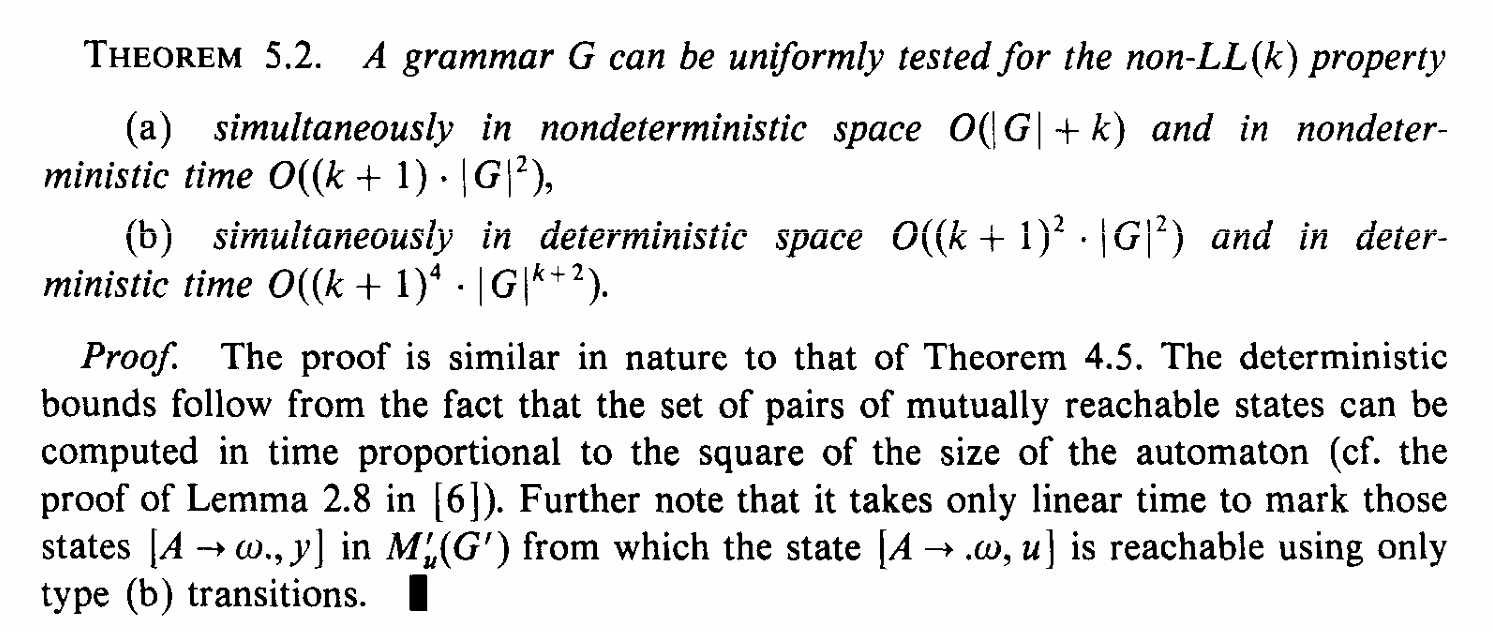
\includegraphics[width=0.5\textwidth]{src/proof.png}
\end{wrapfigure}

It's known that recursive descent parsers may require exponential time in some cases. Although the grammar described in the Introduction is left-recursive, the specific implementation is an $LL(1)$ grammar. The algorithm we implemented is actually a predictive parser, which is a recursive descent syntax analyzer that \textbf{does not require backtracking}. The parser scans the input from left to right, generating the leftmost derivation, and only needs to look ahead one symbol at each step to determine the syntax analysis action. The complexity proof of semantic analysis for $LL(k)$ grammar is shown in Fig~\ref{fig:complexity} (from the paper \textit{On the complexity of $LL(k)$ testing}~\cite{SIPPU1983244}).

\begin{displayquote}
    The algorithm for constructing the canonical $LL(k)$
    parser yields, as a byproduct, a test for the $LL(k)$ property. The problem of testing whether or not a context-free grammar possesses the $LL(k)$ property is studied. For each fixed integer $k \geq 0$, the problem is shown to be solvable in nondeterministic time $O(n)$, and simultaneously in deterministic space $O(n)$ and in deterministic time $O(n^{k+1})$, where n is the size of the grammar in question.
\end{displayquote}

Using the above conclusion, we can conclude that the time and space complexity of our syntax analysis process is $O(n)$.

\subsection{Time and Space Complexity for Optimizer}

The optimizer is described in Alg~\ref{alg:3}. The optimizer will recursively apply the optimization rules to the expression tree. For each node, the optimizer will only execute a constant number of check and assignment operations, so the time complexity of the optimizer is $O(n)$ ($n$ is the number of nodes in the expression tree).

As for space complexity, the optimizer will create a new expression tree, so the space complexity of the optimizer is $O(n)$.

\subsection{Time and Space Complexity for Differentiator}

The differentiator is described in Alg~\ref{alg:4}. The differentiator will recursively apply the differentiation rules to the expression tree.

The difference between the differentiator and the optimizer is that the differentiator may recursively call itself to implement chain rule. I tried to expand the differentiate results so that the differentiator will call itself at most twice for each node (to calculate $f'(x)$ and $g'(x)$). \textbf{On average,} the tree size of two child nodes is about half of the parent node, so the time complexity of the differentiator is:

\begin{displaymath}
    T(n) = 4T(n/2) + O(1)
\end{displaymath}

By master theorem, the time complexity of the differentiator is $O(n^2)$($n$ is the number of nodes in the expression tree).

The space complexity depends on the input expression. If the expression is deeply nested, the result expression will be more complex, so the space complexity will be higher. For example, if you use the expression below for input:

\begin{verbatim}
a^a^a^a^a^a^a^a^a^a^a^a^a^a^a^a^a^a^a^a^a^a^a^a^a^a^a^a^a^a^a^a^a^a^a^a^a^a^a^a^a^a^a^a^a^a
^a^a^a^a^a^a^a^a^a^a^a^a^a^a^a^a^a^a^a^a^a^a^a^a^a^a^a^a^a^a^a^a^a^a^a^a^a^a^a^a^a^a^a^a^a
^a^a^a^a^a^a^a^a^a^a^a^a^a^a^a^a^a^a^a^a^a^a^a^a^a^a^a^a^a^a^a^a^a^a^a^a^a^a^a^a^a^a^a^a^a
^a^a^a^a^a^a^a^a^a^a^a^a^a^a^a^a^a^a^a^a^a^a^a^a^a^a^a^a^a^a^a^a^a^a^a^a^a^a^a^a^a^a^a^a^a
^a^a^a^a^a^a^a^a^a^a^a^a^a^a^a^a^a^a^a^a^a^a^a^a^a^a^a^a^a^a^a^a^a^a^a^a^a^a^a^a^a^a^a^a^a
^a^a^a^a^a^a^a^a^a^a^a^a^a^a^a^a^a^a^a^a^a^a^a^a^a^a^a^a^a^a
\end{verbatim}

Then the result expression tree will have more than 40k nodes. For the worst case like this, we can infer that $S(n) = 2S(n-1) + S(1)$, so space complexity will be $O(2^n)$. On average, the space complexity of the differentiator usually is $O(2n)$ for polynomial expressions, with each node expaned to at most two nodes.

\section{Advantages of the Program}

\begin{itemize}
    \item The program is easy to extend. It is easy to add new operators and functions to the program. The program can also be easily extended to support more complex expressions, such as matrix expressions.
    \item The program is easy to debug and maintain. The program is divided into several modules, and each module is responsible for a specific task. The program can be debugged by testing each module separately and can be easily maintained by modifying each module separately.
    \item The program is easy to use. The program is implemented in C, which is a widely used programming language. The program can be easily compiled and run on most platforms.
\end{itemize}

\section{More on Data Structure}

This program mainly uses tree data structure to store the expression. The tree data structure is suitable for storing expressions because it can represent the hierarchical structure of expressions. But the normal tree data structure also has some disadvantages:

\begin{itemize}
    \item The tree data structure is not very efficient in terms of memory usage.
    \item It's hard to implement some operations on the tree data structure, such as collecting like terms.
\end{itemize}

A more efficient data structure for storing expressions is the DAG (directed acyclic graph) data structure. The DAG data structure can be obtained by removing the duplicate nodes in the expression tree. The DAG data structure can save memory and make some operations more efficient. Nowadays, most compilers use DAG data structure to store and optimize expressions. Fig~\ref{fig:dag} shows an example of building a DAG from infix expressions.

\begin{figure}[!ht]
    \caption{Example of building a DAG from infix expressions.}\label{fig:dag}
    \centering
    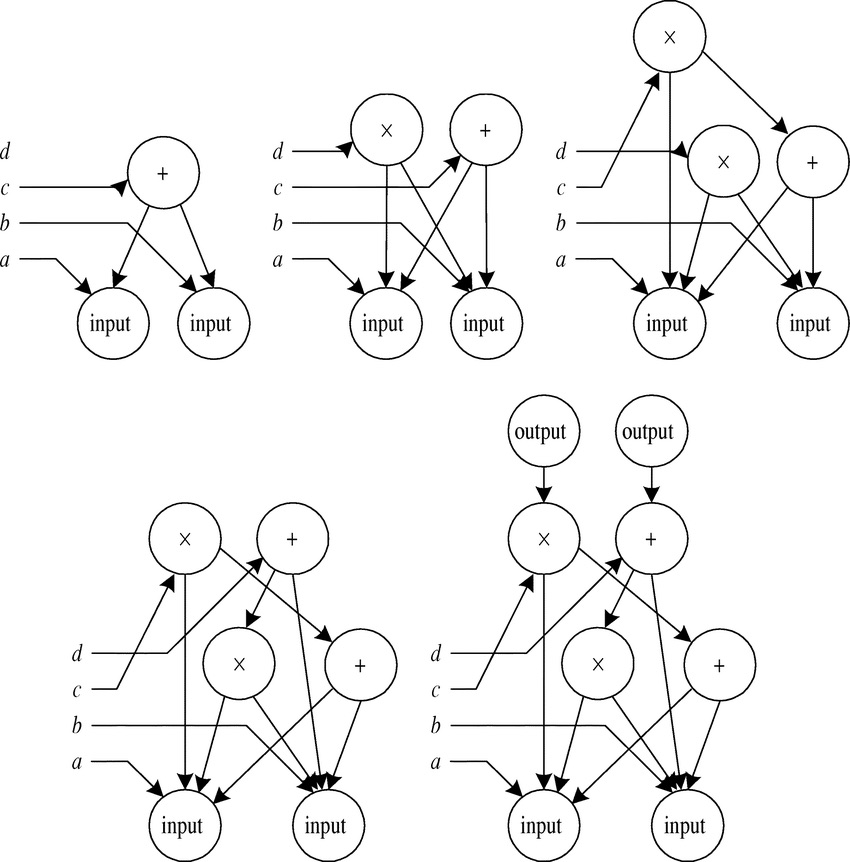
\includegraphics[width=0.6\textwidth]{src/dag.jpeg}
\end{figure}

Using DAG to store expressions can also make some operations more efficient. For example, the \textbf{collecting like terms} operation can be implemented by traversing the DAG and merging the nodes with the same operator and operands. Autograd in DAG is also more efficient. The autograd algorithm in DAG can be implemented by traversing the DAG in the backward direction and merging the nodes with the same operator and operands.

Actually, the DAG data structure is used in the \verb|autograd| module of PyTorch~\cite{paszke2017automatic}. PyTorch is a widely used deep learning framework. The autograd module of PyTorch is used to automatically calculate the gradient of the loss function with respect to the parameters of the neural network. The autograd module uses DAG data structure to store the computation graph of the neural network. The computation graph is a DAG that represents the forward pass of the neural network. The autograd module will automatically calculate the gradient of the loss function with respect to the parameters of the neural network by traversing the computation graph in the backward direction. Fig~\ref{fig:pytorch} shows an example of building a computation graph from a neural network.

\begin{figure}[!ht]
    \caption{Example of building a computation graph from a neural network.}\label{fig:pytorch}
    \centering
    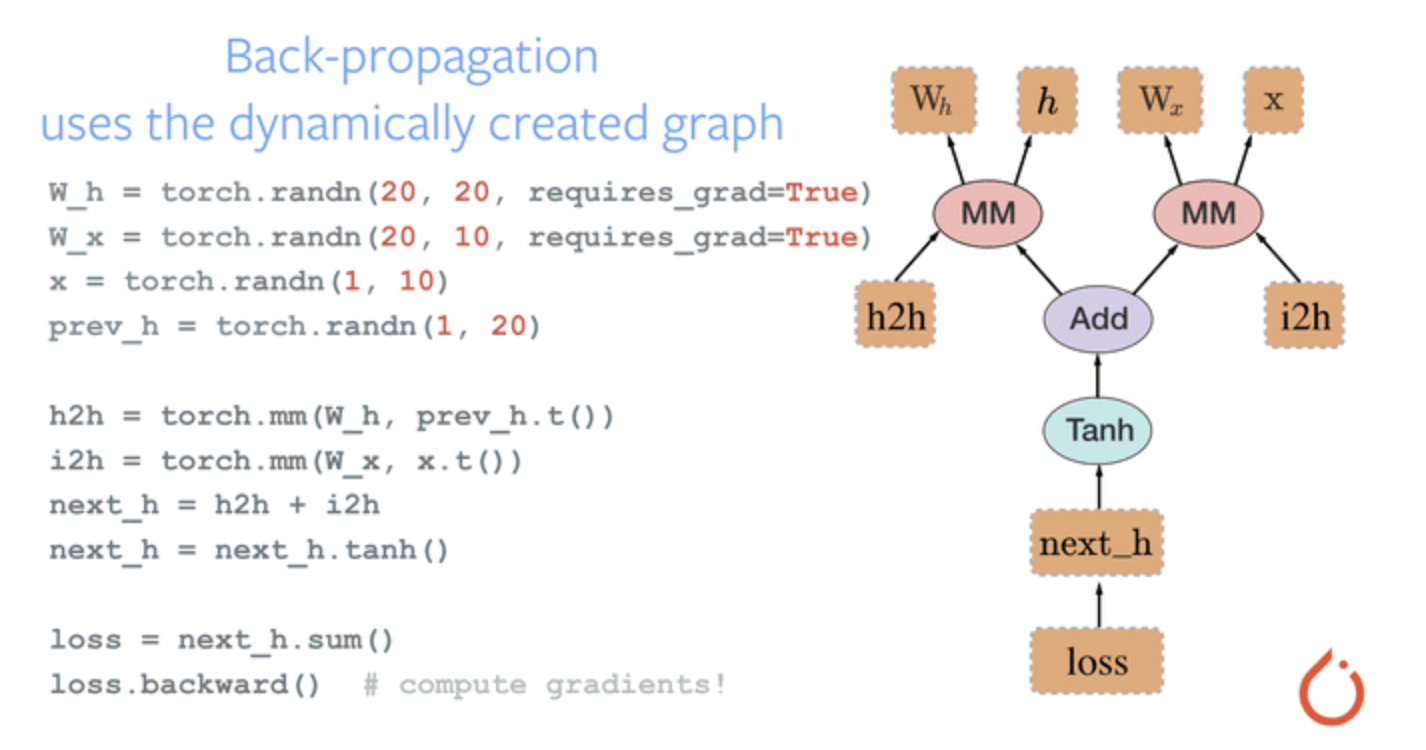
\includegraphics[width=0.6\textwidth]{src/pytorch.png}
\end{figure}

\appendix

\chapter{Source Code}

\section{Source Code Statistics}

The source code is in the \verb|code| directory. I've commented the source code
using Doxygen-style comments.

\begin{enumerate}
    \item \verb|main.c|: Driver program.
    \item \verb|expression.h, expression.c|: Implementation of the expression tree.
\end{enumerate}

And here is the statistics of the source code above using \verb|cloc| tool:

\begin{verbatim}
-------------------------------------------------------------------------------
Language                     files          blank        comment           code
-------------------------------------------------------------------------------
C                                2             58            471           1037
C/C++ Header                     1              9             81             67
-------------------------------------------------------------------------------
SUM:                             3             67            552           1104
-------------------------------------------------------------------------------
\end{verbatim}

$33\%$ of the source code is well documented with Doxygen-style comments. This
satisfies the requirement of the project.

\section{Compilation and Execution}

The program is written in C and can be compiled using \verb|gcc|. There is a \verb|Makefile| in the \verb|code| directory. If you use UNIX system, you can compile the program by running \verb|make| in the \verb|code| directory.

If you use Windows system, you can compile the program by running the following command in the \verb|code| directory:

\begin{verbatim}
gcc -o autoGrad.exe main.c expression.c
\end{verbatim}

If you use IDE, you can also import the source code into the IDE and compile it.

\chapter{Complete Test Suite}
\label{chap:raw_test_results}

Here I present the more detailed test cases and its results.

\section{Test Cases}

Here I classify the test cases into categories:

\begin{itemize}
    \item \textbf{Constant}: Test cases that only contain constants.
          \begin{itemize}
              \item \verb|-1^2|
              \item \verb|(-1)^2|
              \item \verb|1-1+1|
              \item \verb|2*3/3|
          \end{itemize}
    \item \textbf{Simple}: Test cases that only contain variables and constants.
          \begin{itemize}
              \item \verb|x^2+2*x+1|
              \item \verb|a^2+a^2+a^2+b*3+b^2|
              \item \verb|a+(b+c)*d|
              \item \verb|a*b/(a-b)*a/b^2|
              \item \verb|-a|
          \end{itemize}
    \item \textbf{Math Function}: Test cases that contain mathematical functions.
          \begin{itemize}
              \item \verb|sin(x)+cos(x)+tan(x)+exp(x)+ln(x)+log(2, x)+pow(x, 2)|
              \item \verb|pow(x, x)|
          \end{itemize}
    \item \textbf{variable Name}: Test cases that contain variables with different names.
          \begin{itemize}
              \item \verb|vlog+logp|
              \item \verb|a+b+c+d+e+f+g+h+i+j+k+l+m+n+o+p+q+r+s+t+u+v+w+x+y+z|
              \item \verb|abcdefghijklmnopqrstuvwxyz|
          \end{itemize}
    \item \textbf{Complex and Nested}: Test cases that contain nested expressions, multiple variables and functions.
          \begin{itemize}
              \item \verb|xx^2/xy*xy+a^a|
              \item \verb|sin(x+1)*2+cos(x+1)*2|
              \item \verb|log(a,b)^2+sin(x)^2|
              \item \verb|a+(-b)^c|
              \item \verb|log(log(a,b),log(a,b))|
          \end{itemize}
    \item \textbf{Optimization}: Test cases that can be simplified.
          \begin{itemize}
              \item \verb|log(a,a)|
              \item \verb|x+x+x|
              \item \verb|x^0+0^x|
          \end{itemize}
\end{itemize}

\section{Results}

\subsection{Constant}

\begin{verbatim}
> -1^2
No variable in expression: (-1)
> (-1)^2
No variable in expression: 1
> 1-1+1
No variable in expression: 1
> 2*3/3
No variable in expression: 2
\end{verbatim}

\subsection{Simple}

\begin{verbatim}
> x^2+2*x+1
x: x^2*2/x+2
> a^2+a^2+a^2+b*3+b^2
a: a^2*2/a+a^2*2/a+a^2*2/a
b: 3+b^2*2/b
> a+(b+c)*d
a: 1
b: d
c: d
d: b+c
> a*b/(a-b)*a/b^2
a: ((b*(a-b)-a*b)/(a-b)^2*a+a*b/(a-b))*b^2/b^2^2
b: ((a*(a-b)-a*b*(-1))/(a-b)^2*a*b^2-a*b/(a-b)*a*b^2*2/b)/b^2^2
> -a
a: (-1)
\end{verbatim}

\subsection{Math Function}

\begin{verbatim}
> sin(x)+cos(x)+tan(x)+exp(x)+ln(x)+log(2, x)+pow(x, 2)
x: cos(x)+(-1)*sin(x)+1/cos(x)^2+exp(x)+1/x+ln(2)/x/ln(2)^2+x^2*2/x
> pow(x, x)
x: x^x*(1+ln(x))
\end{verbatim}

\subsection{Variable Name}

\begin{verbatim}
> vlog+logp
logp: 1
vlog: 1
> a+b+c+d+e+f+g+h+i+j+k+l+m+n+o+p+q+r+s+t+u+v+w+x+y+z
a: 1
b: 1
c: 1
d: 1
e: 1
f: 1
g: 1
h: 1
i: 1
j: 1
k: 1
l: 1
m: 1
n: 1
o: 1
p: 1
q: 1
r: 1
s: 1
t: 1
u: 1
v: 1
w: 1
x: 1
y: 1
z: 1
> abcdefghijklmnopqrstuvwxyz
abcdefghijklmnopqrstuvwxyz: 1
\end{verbatim}

\subsection{Complex and Nested}

\begin{verbatim}
> xx^2/xy*xy+a^a
a: a^a*(1+ln(a))
xx: xx^2*2/xx*xy/xy^2*xy
xy: (-1)*xx^2/xy^2*xy+xx^2/xy
> sin(x+1)*2+cos(x+1)*2
x: cos(x+1)*2+(-1)*sin(x+1)*2
> log(a,b)^2+sin(x)^2
a: log(a,b)^2*(-1)*ln(b)/a/ln(a)^2*2/log(a,b)
b: log(a,b)^2*ln(a)/b/ln(a)^2*2/log(a,b)
x: sin(x)^2*cos(x)*2/sin(x)
> a+(-b)^c
a: 1
b: ((-1)*b)^c*(-1)*c/(-1)*b
c: ((-1)*b)^c*ln((-1)*b)
> log(log(a,b),log(a,b))
a: (0)
b: (0)
\end{verbatim}

\subsection{Optimization}

\begin{verbatim}
> log(a,a)
a: (0)
> x+x+x
x: 3
> x^0+0^x
x: (0)
\end{verbatim}

\bibliography{report}

\end{document}